% Compile with latex, then dvisvgm --no-fonts --exact --bbox=min.
\documentclass[tikz,border=5pt]{standalone}
\begin{document}
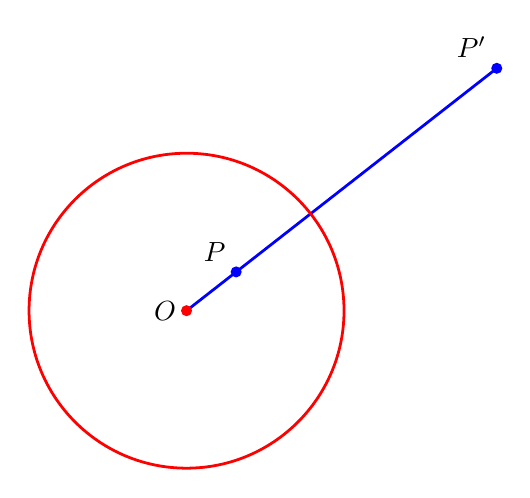
\begin{tikzpicture}[line width=1pt]
  % OP = 0.8, OP' = 5, so OP * OP' = R^2 = 4.
  \coordinate (O) at (0,0);
  \coordinate (P) at (38:0.8);
  \coordinate (Q) at (38:5);
  \draw[blue] (O) -- (Q);
  \draw[red] (O) circle (2);
  \fill[red] (O) circle (2pt) node[left,black] {$O$};
  \fill[blue] (P) circle (2pt) node[above left,black] {$P$};
  \fill[blue] (Q) circle (2pt) node[above left,black] {$P'$};
\end{tikzpicture}
\end{document}
